Идея данного метода балансировки достаточно проста.
Батарея состоит из нескольких последовательных блоков и ключей.
Ключи установленны таким образом, чтобы включать/выключать конкретную ячейку из общей сети.

\begin{figure}[!h]
    \centering
    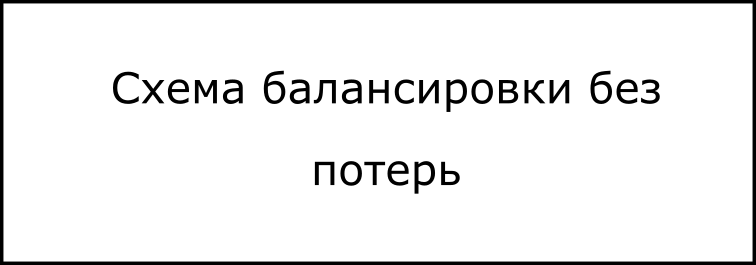
\includegraphics[width=0.7\linewidth]{img/no_loss_balancing.png}
    \caption{Принципиальная схема для балансировки "без потерь"}
    \label{fig:no_loss}
\end{figure}
